\documentclass[11pt]{beamer}
\usepackage[utf8]{inputenc}
\usepackage[T1]{fontenc}
\usepackage[portuguese]{babel}
\usepackage{amsmath}
\usepackage{amsfonts}
\usepackage{amssymb}
\usepackage{graphicx}
\usetheme{CambridgeUS}
\usepackage{adjustbox}
\setbeamertemplate{footline}[page number]
\begin{document}
	\author{Bruno Ferrari Guide}
	\title{Perspectivas na Análise de Textos Não-Estruturados}
	%\subtitle{}
	%\logo{}
	\institute[DL - USP]{
\includegraphics[width=3cm]{Glic.png}\\
	\medskip
	\textit{bruno.fguide@gmail.com} % Your email address
}
	\date{22 de Novembro de 2017}
	%\subject{}
	%\setbeamercovered{transparent}
	%\setbeamertemplate{navigation symbols}{}
	\begin{frame}[plain]
	\maketitle
\end{frame}

\begin{frame}
\frametitle{Índice} % Table of contents slide, comment this block out to remove it
\tableofcontents % Throughout your presentation, if you choose to use \section{} and \subsection{} commands, these will automatically be printed on this slide as an overview of your presentation
\end{frame}

\section{Introdução - A importância dos dados}
%0.1 linguistica computacional e a importância dos dados
%0.2 grande quantidade de informações disponíveis
%0.3 modelos cada vez mais data driven...



\begin{frame}
\frametitle{Introdução}
\begin{itemize}
	\item Textos são conjuntos de dados linguísticos.\\
	\item Textos não-estruturados significam dados não estruturados.\\
	\item Por que os dados são tão centrais para a Linguística Computacional?\\
	\item Por que chamamos esse tipo de dado de não-estruturado?\\
\end{itemize}
\end{frame}

\begin{frame}
\frametitle{Importância dos dados para a Linguística Computacional}
\begin{itemize}
	\item Da wikipedia: \textit{Computational linguistics is an interdisciplinary field concerned with the statistical or rule-based modeling of natural language from a computational perspective, as well as the study of appropriate computational approaches to linguistic questions.}\\
\end{itemize}
\end{frame}

\begin{frame}
\frametitle{Modelos Baseados em Regras}
\begin{itemize}
	\item Modelos baseados em regras são construídos a partir de um conjunto de instruções que descrevem um determinado fenômeno.\\
	\item Exemplo: Plural do Português $\rightarrow$ 's' no fim da palavra caso termine em vogal, 'es' caso termine em consoante.\\
	\item Caso não funcione, se cria uma exceção que deve ser tratada com regras diferentes.\\
\end{itemize}
\end{frame}

\begin{frame}
\frametitle{Modelos Probabilísticos}
\begin{itemize}
	\item Modelo probabilístico é baseado na observação de uma amostra de dados que representem um determinado processo. A partir dessa amostra o modelo tentará capturar o comportamento do processo. O modo como isso será feito define o tipo de modelo.\\
	\item \textbf{Exemplo - }Observação: A partir do estudo de 100 palavras no singular e sua forma plural, temos 90\% que fazem o plural com a adição de 's' no fim da palavra, 5\% com a adição de 'es' e 3\% como em 'pão' - 'pães' e 2\% como em 'lápis' - 'lápis'.\\
	\item Modelo: lista o conjunto de sílabas finais da amostra e associa a cada um deles a probabilidade dele seguir um dos 4 padrões observados.\\
\end{itemize}
\end{frame}


\begin{frame}
\frametitle{Modelos Baseados em Regras vs. Probabilísticos}
\begin{itemize}
	\item Modelos baseados em regras ainda existem, mas no mundo da NLP, desde os anos 80, os principais modelos computacionais para linguagem natural são probabilísticos.\\
	\item Além disso, a soma de dois fatores, explosão de dados disponíveis e grande poder de processamento acessível, mostram que é muito improvável que esse cenário se reverta nos próximos anos.\\
\end{itemize}
\end{frame}

\section{Dados Estruturados vs. Dados não-Estruturados}
%1.1 - Definição de dados estruturados
%1.2 - Exemplo
%1.3 - Mundo real: Exemplo de dados não-estruturados
%1.4 - Tabela comparando coisas como disponibilidade, organização, previsibilidade.
%1.5 - Para construir qualquer aplicação, é necessário estruturar o dado linguístico. A área de processamento de linguagem natural é justamente isso.
\begin{frame}
\begin{center}
\textbf{Dados Estruturados e Dados não-Estruturados}
\end{center}
\end{frame}
\begin{frame}
\frametitle{Dados Estruturados e Não-Estruturados}
\begin{itemize}
	\item Dados estruturados são aqueles que tem um formato especificado, em que as informações relevantes estão dispostas de modo organizado. É possível fazer inferências sobre eles.\\
	\item Os dados não-estruturados dependem de pré-processamento para que as informações relevantes sejam extraídas.\\ 
	
\end{itemize}
\end{frame}

\begin{frame}
\frametitle{Exemplo de dados Estruturados}
\begin{center} 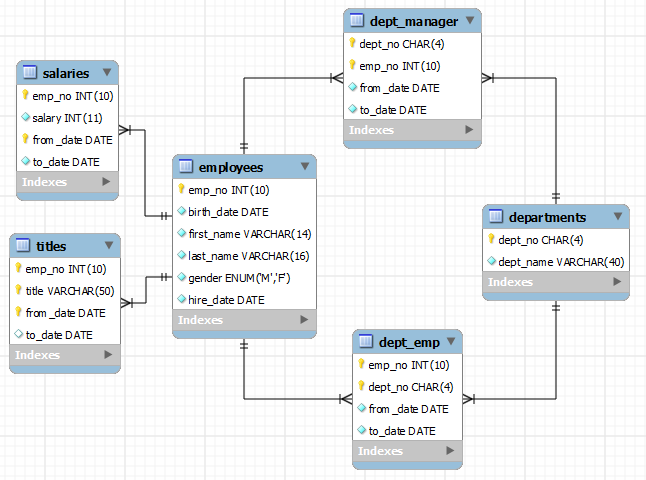
\includegraphics[width=\linewidth,height=\textheight,keepaspectratio]{DadosEstruturados.png}
\end{center}
\end{frame}

\begin{frame}
\frametitle{Exemplo de dados não-estruturados}
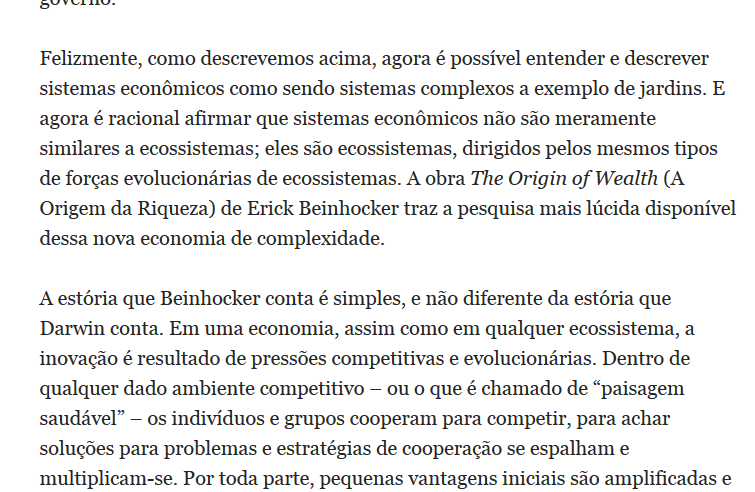
\includegraphics[width=5cm,height=5cm,keepaspectratio]{texto_data.png}
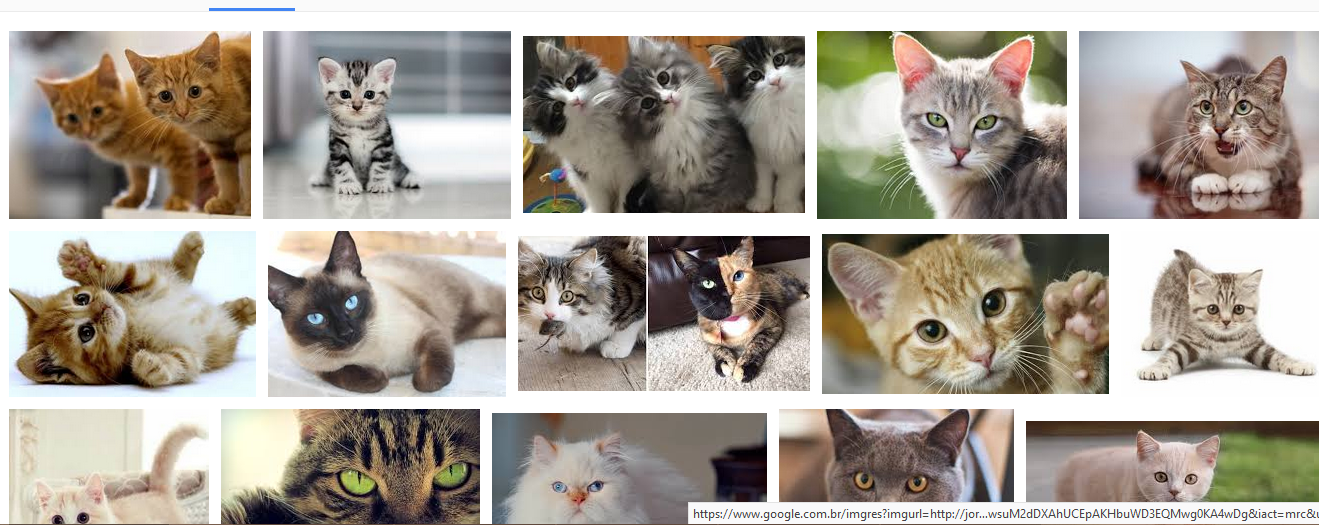
\includegraphics[width=5cm,height=5cm,keepaspectratio]{ibagens_data.png}
\end{frame}

\begin{frame}
\frametitle{Dados Estruturados vs. Dados não-Estruturados}
	\begin{table}[]
		\centering
		
		\label{my-label}
		\resizebox{\textwidth}{!}{%
			\begin{tabular}{l|l}
				\hline
				Dados estruturados & Dados não-estruturados \\ \hline
				Menor quantidade disponível & Imensa disponibilidade \\
				Informações organizadas e prontas para serem procesadas & Exige pré-processamento para extração de informações relevantes \\
				&  \\ \hline
			\end{tabular}%
		}
	\end{table}
\end{frame}

\begin{frame}
\frametitle{Processamento de Linguagem Natural}
\begin{itemize}
	\item Para construir qualquer aplicação usando dados linguísticos, é necessário estruturar esses dados.\\
	\item Há esforços para conseguir estruturar os mais diversos aspectos da língua para criar modelos que consigam fazer inferências sobre dados linguísticos.\\
\end{itemize}
\end{frame}


\section{Língua e Estrutura}

\begin{frame}
\begin{center}
	Língua e estrutura
\end{center}
\end{frame}
%GRANDE DISCLAIMER - Dado estruturado != Estrutura interna da língua [interna em termos de 'Estrutura atribuída ao sistema linguístico'].
%2.1- Maas, o modo de tornarmos o dado linguístico não estruturado em um dado bonito e processável pode se apoiar na estrutura interna da língua.
%2.2 - Isso é maravilhoso na teoria, parcerias entre linguistas e computeiros. Mas a estrutura interna da língua é um caos. Complexa pra caramba, ambígua até o osso, não monotônica, quanto mais você afunda, mais ela afunda... O que fazer com isso
%2.3- É importante diferenciar estruturações 'Deep' e 'Shallow'. Exemplo de análise 'deep' e análise 'shallow' de uma sentença.
\begin{frame}
\frametitle{A língua não tem estrutura?}
\begin{itemize}
	\item Importante: Não há relação entre a estrutura interna do fenômeno que gera um dado e o fato deste dado estar estruturado ou não.\\
	\item No entanto, a estrutura interna do fenômeno pode ser bastante útil para organizar e padronizar os dados observados.\\
\end{itemize}
\end{frame}
\begin{frame}
\frametitle{Como essa estrutura é útil para o processamento?}
\begin{itemize}
	\item Exemplo: previsão da próxima palavra dada a palavra anterior.\\
	\item  \textbf{o pai do ???\\}
	\item É muito difícil fazer a previsão da próxima palavra, no entanto é bem possível que a gente faça previsões sobre algumas características da palavra que falta, como sua categoria morfossintática, gênero, número.\\
	
\end{itemize}
\end{frame}
\begin{frame}
\frametitle{Porém...}
\begin{itemize}
	\item <1-> A estrutura interna da língua é um tipo de diferente do desejado para os chamados dados estruturados. É muito mais complexa, o que torna a relação entre a estrutura interna e os dados estruturados algo não trivial.\\
	\item <2-> Ambiguidades estruturais são comuns na língua e um pesadelo na estruturação de dados.\\
	\item <3->Devido a essa grande complexidade da estrutura linguística, é bastante recorrente no campo da Lx. Computacional modelar a língua desconsiderando a estrutura problemática.\\
	\item <4->O simples reconhecimento de padrões \textit{superficiais} nos dados linguísticos já é algum tipo de análise linguística.\\
	
	
\end{itemize}
\end{frame}

\section{Alguns métodos}
%3.1- Expressões Regulares
%3.2- Lematização
%3.3- Tokenização
%3.4- POS-Tagging
%3.5- Semantic Role Labelling
\begin{frame}
\begin{center}
	Alguns métodos para estruturar dados linguísticos
\end{center}
\end{frame}
\begin{frame}
\frametitle{Expressões Regulares - Regex}
\begin{itemize}
	\item \textbf{O que é:} Método para reconhecer sequências de caracteres. Permite que sejam encontrados tipos de caracteres específicos, repetições.\\
	\item \textbf{Utilidade:} Extremamente útil para extrair palavras-chave, capturar pequenas variações de expressões. Ferramenta poderosa.\\
	\item Quanto da estrutura linguística é representada nas Regex?
\end{itemize}
\end{frame}
\begin{frame}
\frametitle{Expressões Regulares - Exemplo}
\begin{center}
	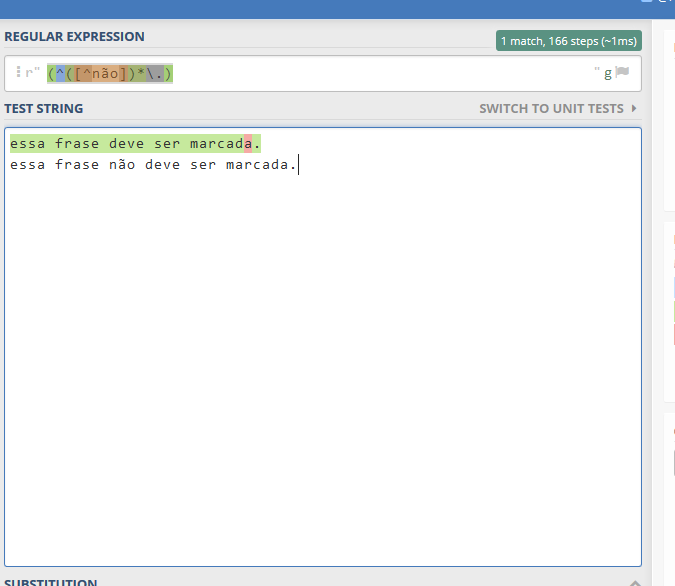
\includegraphics[width=\columnwidth,height=\textheight,keepaspectratio]{Regex_bom.png}
\end{center}
\end{frame}

\begin{frame}
\frametitle{Expressões Regulares - Exemplo}
\begin{center}
	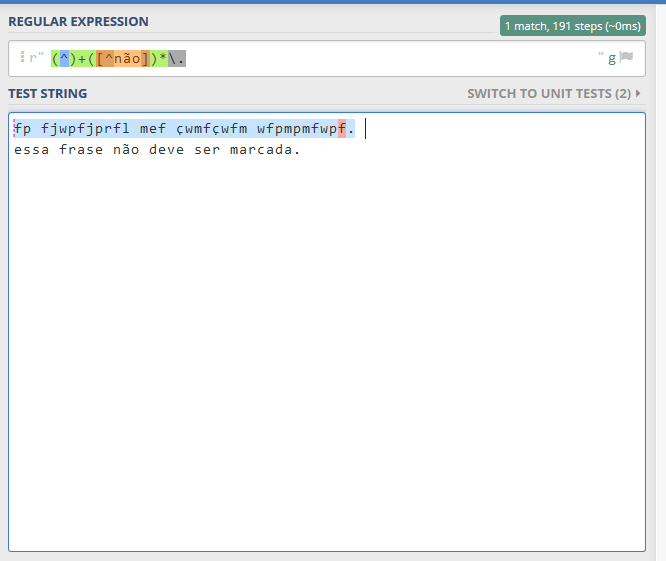
\includegraphics[width=\columnwidth,height=\textheight,keepaspectratio]{Regex_ruim.png}
\end{center}
\end{frame}


\begin{frame}
\frametitle{Lematização}
\begin{itemize}
	\item \textbf{O que é:} Traduzir as formas morfológicas diversas de uma palavra para sua versão dicionarizada (lema).\\
	\item \textbf{Utilidade:} Reduz a riqueza de formas da língua enquanto mantém algumas informações, preserva alguma parte do significado.\\
\end{itemize}
\end{frame}

\begin{frame}
\frametitle{Lematização - Exemplo}
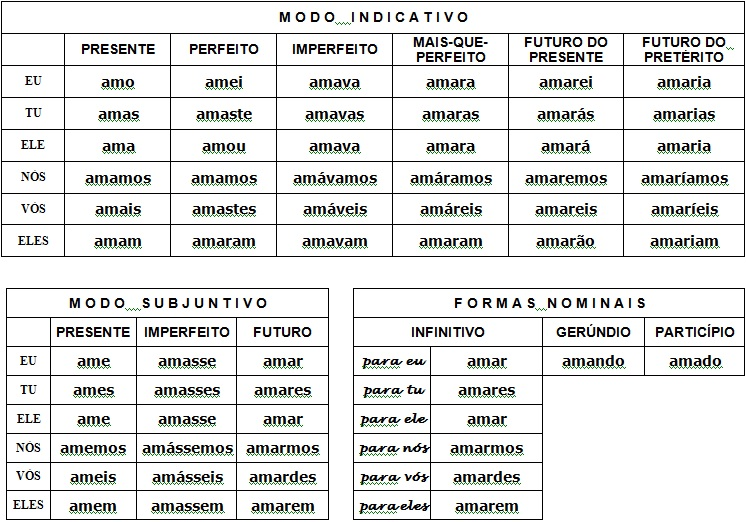
\includegraphics[width=\columnwidth,height=\textheight,keepaspectratio]{verbos.jpg}
\end{frame}

\begin{frame}
\frametitle{Lematização - Exemplo}
\begin{center}
	\large amar
\end{center}
\end{frame}


\begin{frame}
\frametitle{POS-Tagging}
\begin{itemize}
	\item \textbf{O que é:} Etiquetar a categoria morfossintática de palavras.\\
	\item \textbf{Utilidade:} Reduz MUITO a diversidade dos dados, mantém algum tipo de informação linguística que pode ser útil para algumas generalizações. Perde muita informação também.\\
\end{itemize}
\end{frame}


\begin{frame}
\frametitle{POS-Tagging - Exemplo}
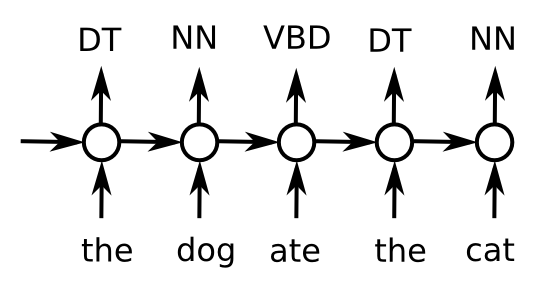
\includegraphics[width=\columnwidth,height=\textheight,keepaspectratio]{pos_tag.png}
\end{frame}


\section{Alguns problemas}
%4.1 - Todos eles erram e a linguagem consegue facilmente quebrar qualquer sistema que a estruture nesses moldes.
%4.2 - Exemplos de erros
%4.3 - Estado da arte em algumas áreas
%4.4 - Noção de acerto - 90% de acerto é o suficiente?
\begin{frame}
\begin{center}
	Alguns problemas para estruturar dados linguísticos
\end{center}
\end{frame}
\begin{frame}
\frametitle{"All grammars leak"}
\begin{itemize}
	\item <1-> Exceções, coisas estranhas, comportamentos opostos dentro da mesma língua.\\
	\item <2-> Além disso, diversos dos algoritmos que fazem as tarefas de estruturação que eu apresentei são probabilísticos e por isso o erro é algo que faz parte dessas abordagens.\\
	\item <3-> Portanto, essa estruturação de dados é sempre complexa e falha. Existem alternativas para lidar com isso (revisão e/ou diluição de erros).\\
\end{itemize}
\end{frame}
\begin{frame}
\frametitle{Estado da arte em algumas áreas}
\begin{itemize}
	\item Regex - não há.\\
	\item Lematização - Inglês (93\%), Português (97\%).\\
	\item POS Tagging - Inglês (85.85\% para itens não vistos e 96.46\%), Português (85\%?).\\
\end{itemize}
\end{frame}
\begin{frame}
\frametitle{O que significam estes índices de acerto?}
\begin{itemize}
	\item O número sem a metodologia da avaliação acaba sendo meio vazio. Por exemplo, as palavras foram consideradas isoladas ou em contexto? Em inglês isso é fundamental para considerar a tarefa de pos-tagging, por exemplo.\\
	\item Se 90\% das palavras estão classificadas corretamente, quer dizer que em uma sentença de 10 palavras uma delas estará errada, logo a sentença não irá ser representada do jeito correto (100\% errada!).\\
\end{itemize}
\end{frame}

\section{Estudo de caso 1: B.Os}
\begin{frame}
\begin{center}
	Estudos de Caso \footnote{Atenção: Eles são deprimentes.}
\end{center}
\end{frame}
\begin{frame}
\frametitle{Contexto do projeto}
\begin{itemize}
	\item Lei de Transparência obriga uma certa organização de segurança pública a divulgar determinados tipos de Boletins de Ocorrência.\\
	\item A divulgação é feita de forma não estruturada, apesar dos dados internamente estarem estruturados.\\
	\item O objetivo do projeto foi justamente estruturar os dados linguísticos contidos nos B.Os.\\
\end{itemize}
\end{frame}
\begin{frame}
\frametitle{Contexto do projeto}
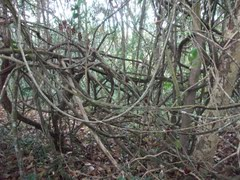
\includegraphics[width=\columnwidth,height=\textheight,keepaspectratio]{Cipoal.jpg}
\end{frame}
\begin{frame}
\frametitle{Os dados}
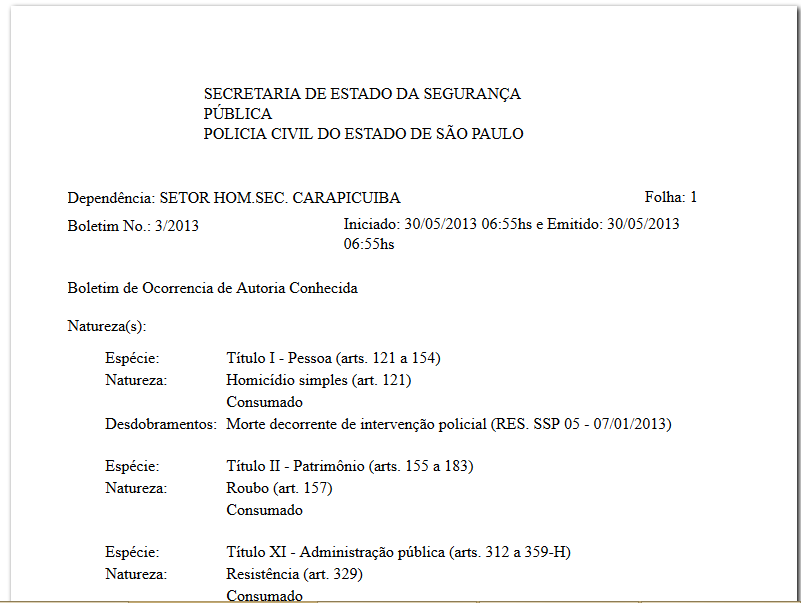
\includegraphics[width=\columnwidth,height=\textheight,keepaspectratio]{bo-bonito.png}
\end{frame}
\begin{frame}
\frametitle{Os dados}
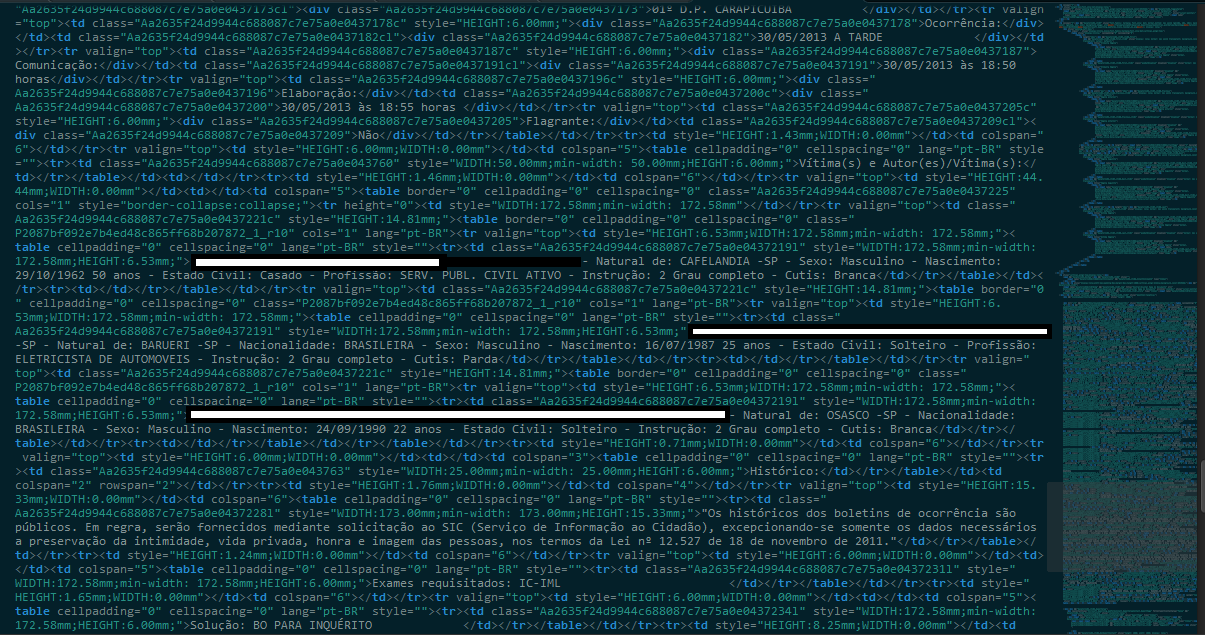
\includegraphics[width=\columnwidth,height=\textheight,keepaspectratio]{bo-html.png}
\end{frame}
\begin{frame}
\frametitle{Método}
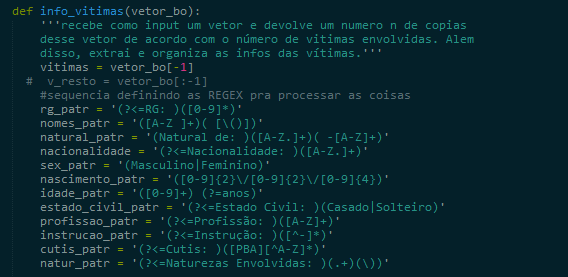
\includegraphics[width=\columnwidth,height=\textheight,keepaspectratio]{bo-regex.png}
\end{frame}
\begin{frame}
\frametitle{Resultados}
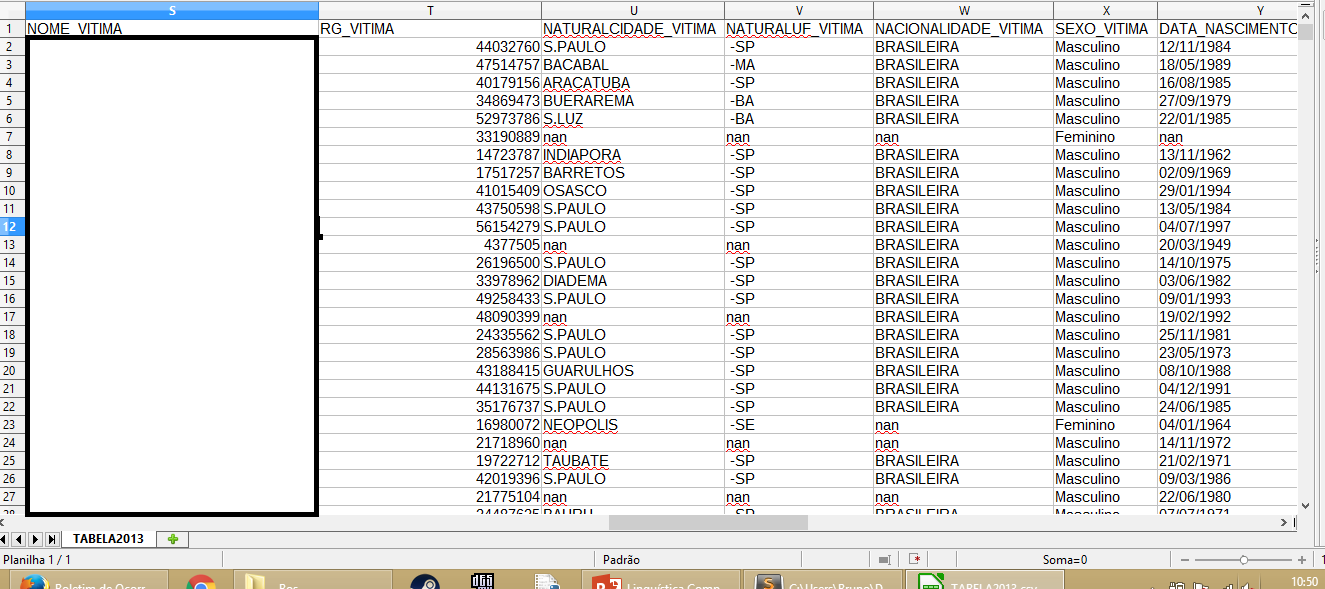
\includegraphics[width=\columnwidth,height=\textheight,keepaspectratio]{bo-excel.png}
\end{frame}

\section{Estudo de caso 2: Projeto Cipoal}
\begin{frame}
\frametitle{Contexto do projeto Cipoal}
\begin{itemize}
	\item \textbf{Corpus: }Leis aprovadas pela câmara dos vereadores do município de São Paulo.\\
	\item \textbf{Problema: }Conjunto de dados grande, armazenado de um jeito caótico, mídias diferentes.\\
	\item Para propor \textit{qualquer} novo projeto de lei, é necessário ver se o projeto entra em conflito com leis anteriores, ver se ele já não foi proposto, etc...\\
\end{itemize}
\end{frame}
\begin{frame}
\frametitle{Os dados}
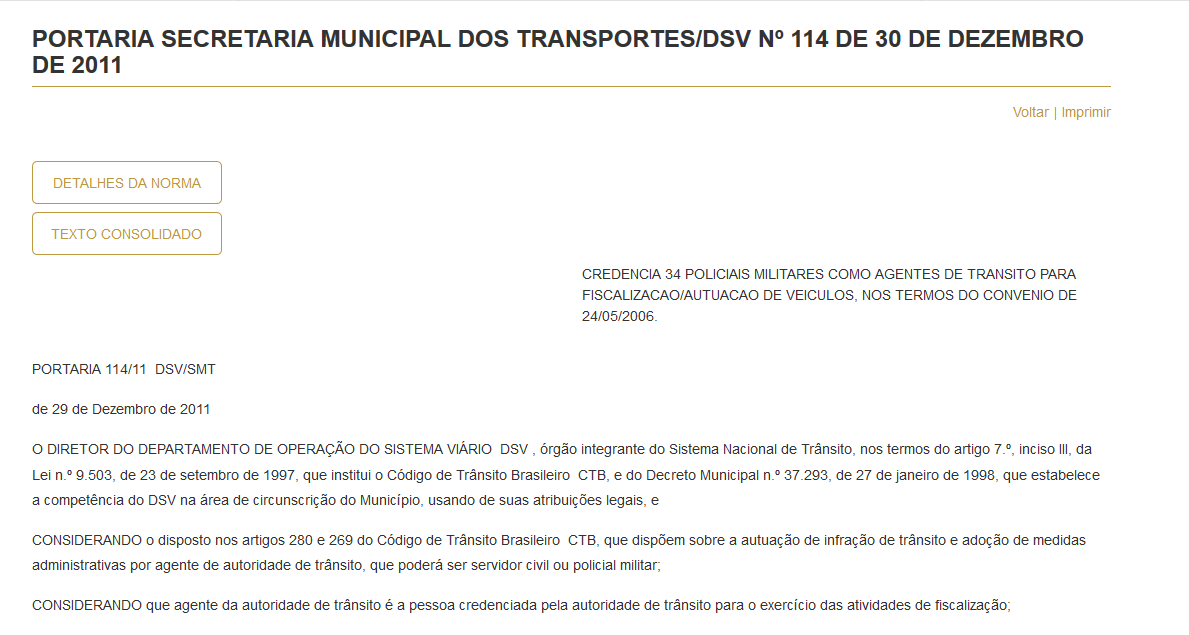
\includegraphics[width=\columnwidth,height=\textheight,keepaspectratio]{Lei_site.png}
\end{frame}
\begin{frame}
\frametitle{Método}
\begin{itemize}
	\item <1-> Neste primeiro momento: Estruturar o corpus e classificar o projeto de lei com Expressões Regulares.\\
	\item <2->Para estruturar: identificar os padrões linguísticos que determinam o que é o cabeçalho, as normas de citação de outras leis e projetos, valores.\\
	\item <3->Para classificar: primeiro, definir as classes relevantes, depois relacionar com palavras-chave e expressões multi-palavra que identifiquem as coisas a serem classificadas.\\
\end{itemize}
\end{frame}
\begin{frame}
\frametitle{Resultados Parciais}

\includegraphics[width=\columnwidth,height=\textheight,keepaspectratio]{Cipoal1.jpg}
\end{frame}
\begin{frame}
\frametitle{Resultados Parciais}
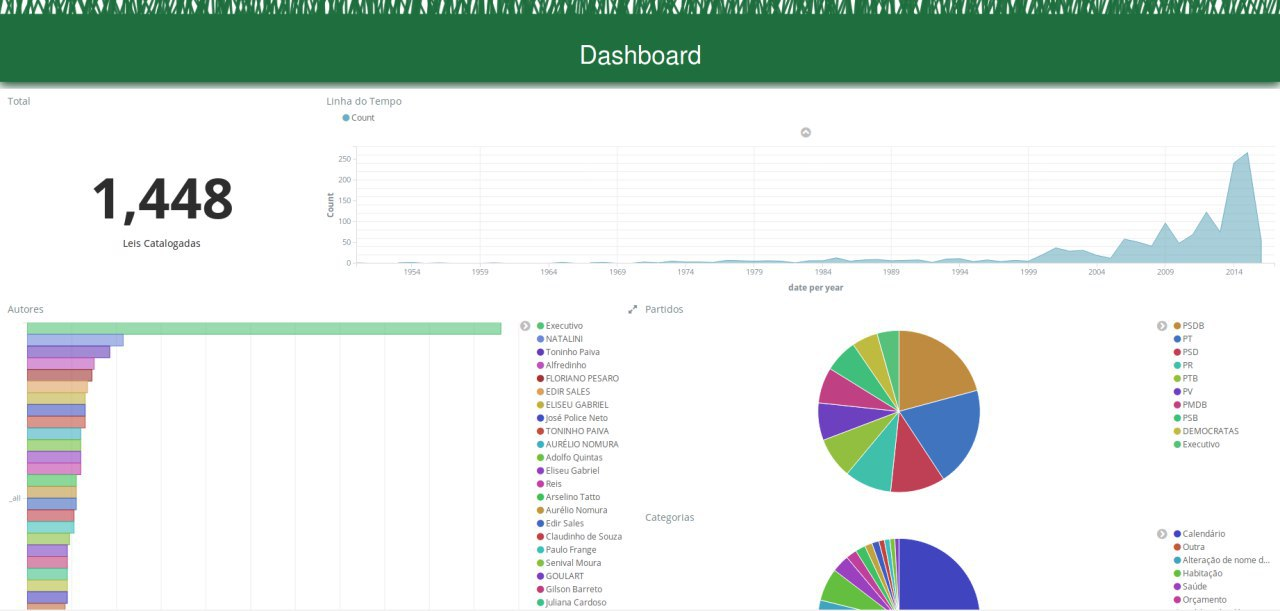
\includegraphics[width=\columnwidth,height=\textheight,keepaspectratio]{Cipoal2.jpg}

\end{frame}
\begin{frame}
\frametitle{Resultados Parciais}
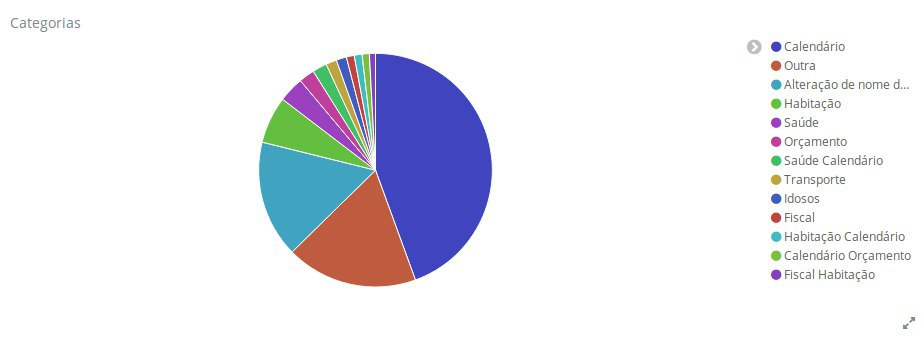
\includegraphics[width=\columnwidth,height=\textheight,keepaspectratio]{CipoalCat.jpg}

\end{frame}
\begin{frame}
\frametitle{Resultados Parciais}
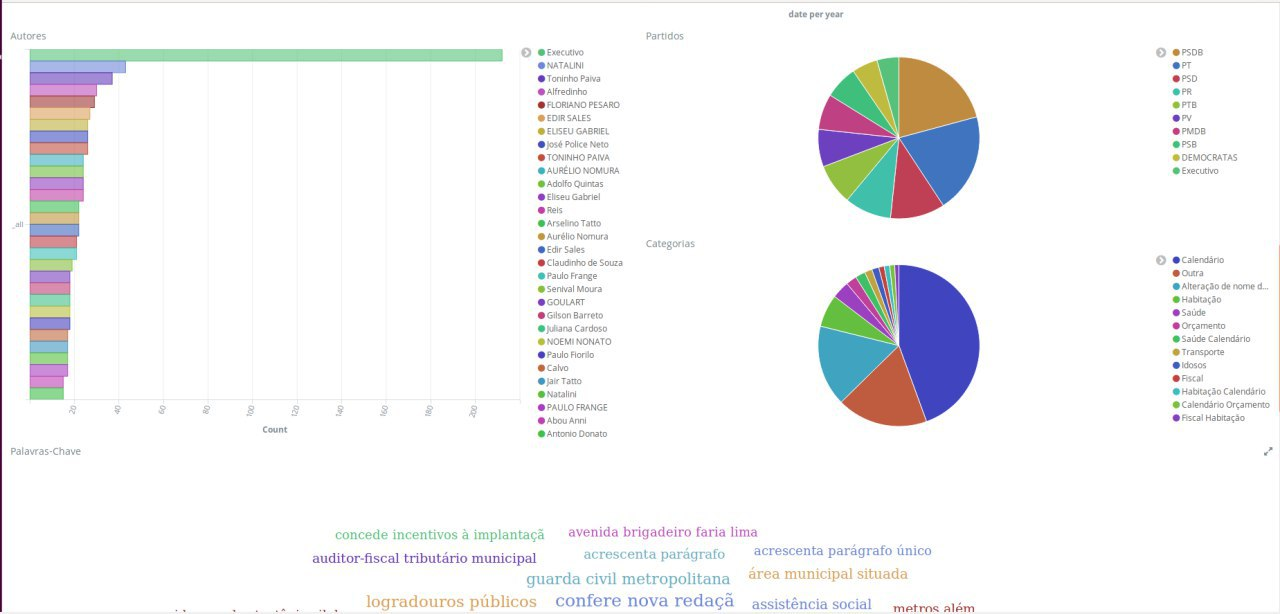
\includegraphics[width=\columnwidth,height=\textheight,keepaspectratio]{Cipoal3.jpg}

\end{frame}
\begin{frame}
\frametitle{Resultados Parciais}
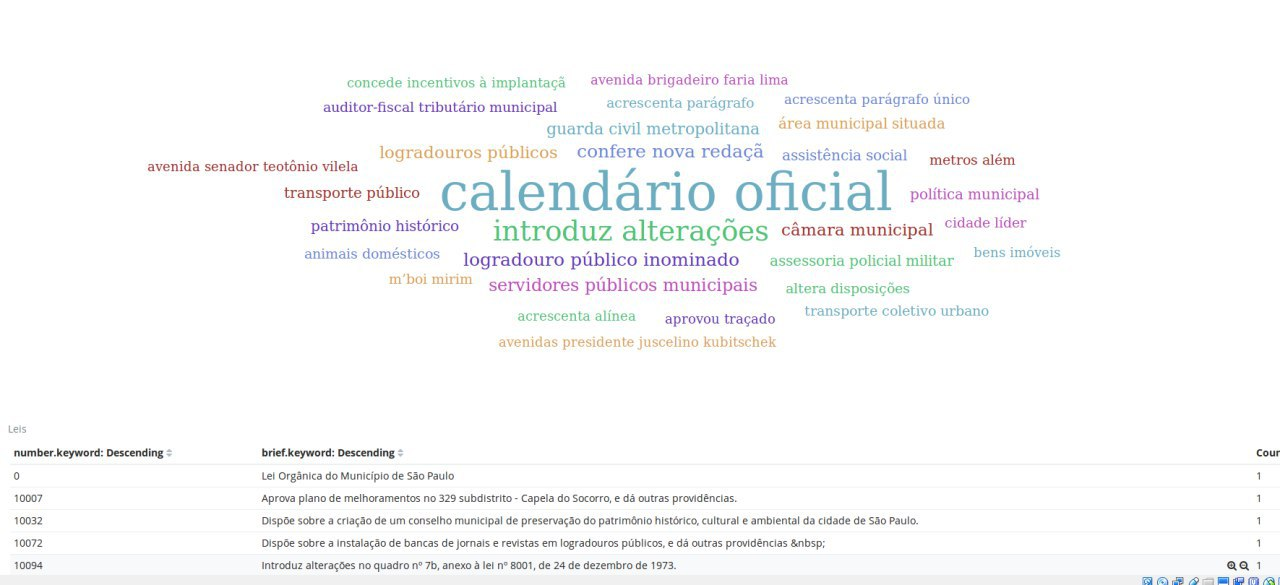
\includegraphics[width=\columnwidth,height=\textheight,keepaspectratio]{Cipoal4.jpg}

\end{frame}
\begin{frame}
\frametitle{Contato}
\begin{center}
	Muito obrigado!\\
	bruno.fguide@gmail.com
\end{center}
\end{frame}
\end{document}

%Bibliografia
% acl wiki
% resultado do pos tagger
% jurafsky
% manning sobre erros
% wiki - dados e ling comp.
% chomsky - estruturas sintáticas
% 